%----------------------------------------------------------------------------------------
%	Software
%----------------------------------------------------------------------------------------

\chapter{Software Components}
\section{Embedded}
\subsection{Firmware Implementation Structure}
The functionality requirements of the embedded firmware was split into its respective files - this improved modularity and readability of code. The firmware will be running on a Raspberry Pi Pico W which will control the main operation of the scale. The three main parts will be the ADC controller, the finite state machine (FSM), and the network interface. 

\textbf{The C file structure is as follows:} 
\textbf{pico\_c.c} contains main code that initialises all relevant functions and contains the FSM; \textbf{functions.c} contains helper functions related to weight calculations; \textbf{led.c} contains LED related functions; \textbf{network.c} contains the TCP/IP/HTTP related functions; \textbf{adc.c} contains ADC conversion related functions.

\textbf{Power saving considerations}: RegEn pin is set to low when we are sending data to the server (this controls the linear regulator, which, when set to low cuts the power to the rest of the circuit). This occurs during the send\_data state as this usually takes 5-8 seconds and our system is blocked until this process is complete. Thus we deemed it an efficient way to save power. We did not implement a sleep mode for when the system was not in use for a pro-longed period of time as our use case assumed the weighing scales would be turned off after, so we did not believe it was necessary. 

\textbf{Debugging and testing}: Testing of firmware was carried out by printf statements and reading the serial outputs. Sleep functions were used where necessary to slow down execution. 

\subsection{General-Purpose Input/Output Port Mapping}
The scale is able to effectively show the user its current status of the system through the use of four LEDs: power, wifi connectivity, stable weight, and tare activation. The mapping of all GPIO ports on the Raspberry Pico W with  the LEDs, Tare Button, and Regulator Enable are shown in the following:

\begin{center}
    \textbf{GPIO Pins used on the Raspberry Pico W} 
\end{center}
\begin{table}[h]
    \centering
    \begin{tabular}{|c|c|}
        \hline
        Pin Type & GPIO Pin \\
        \hline
        Power LED & GP16 \\
        Wi-Fi LED & GP17 \\
        Stable LED & GP18 \\
        Tare LED & GP19 \\
        Tare Button & GP20 \\
        RegEn Pin & GP28 \\
        \hline
    \end{tabular}
    \caption{GPIO Pins Used}
    \label{tab:gpio_table}
\end{table}

\textbf{The mapping of LEDs + RegPin to the FSM states are as follows:}
\begin{itemize}
    \item idle → turn on Reg Pin
    \item not\_ready → turn on Power LED
    \item ready → turn on Wi-Fi LED
    \item tare\_intialized → turn on/off Tare LED
    \item receive\_data → turn on Stable LED
    \item send\_data → turn off RegEn Pin, turn off Stable LED
\end{itemize}

\subsection{Finite State Machine}
The Finite State Machine (FSM) consists of 6 different states (idle, not\_ready, ready, tare\_initialized, receive\_data, send\_data). The data inputs into the system occurs during the polling stage in the idle state. Here the system can transition state based on either a stable weight reading or high tare flag which is set by the tare button Interrupt Service Routine (ISR).

\begin{enumerate}
    \item idle state: The system is polling for data inputs: either a stable weight from the weighing scale or a tare flag from the tare button ISR
    \item not\_ready state: Turns on the Power LED to indicate that the power is turned on, however WiFi is not enabled 
    \item ready\_state: Once Wi-Fi is successfully connected, a initial offset calibration is calculated. This is due to potential zeroing issues of the actual scale hardware. Once this process is complete, both Power and Wi-Fi LEDs are enabled.
    \item tare\_initialized state: When the user pushes the tare button, the ISR set the tare flag to high. This is detected by the idle state which transitions to this state. Tare LED is enable while the tare offset is calculated and applied to the current weight reading. Once this is finished, Tare LED is turned off.
    \item receive\_data state: This state contains a fail safe where it checks for invalid weights. If the weight is below a certain threshold (0.30 Kg in our product), the weight data is not sent to server and state transitions back to idle. This is to prevent negative and zero weight readings being sent to the server. Stable LED is turned on.
    \item send\_data state: Once the weight is determined to be valid, it is sent to the backend server. The stable LED is turned off once this process is complete.
\end{enumerate}

\begin{figure}[h]
    \centering
    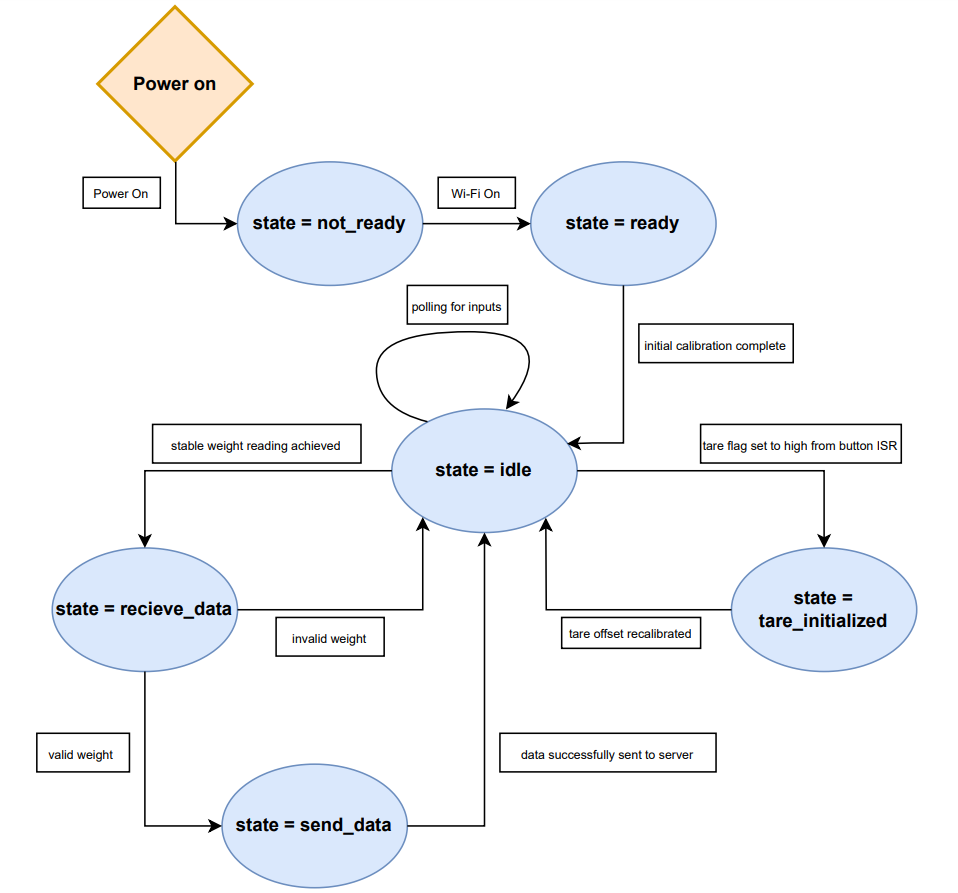
\includegraphics[width=0.9\textwidth]{final-report/assets/770_FSM.PNG}
    \caption{FSM Diagram}
    \label{fig:FSM_diagram}
\end{figure}

\subsection{ADC Reading and Averaging Methodology}
\textbf{ADC Conversion}\\
The Pico W has a 32-bit ADC therefore there are a total of 4096 possible values. The ADC range is 0-3.3V, therefore our resolution for each step can be calculated with 3.3/(4096 - 1). These calculations are performed by the defined macros: $ADC\_RANGE = (1 << 12)$ and $ADC\_CONVERT = (3.3 / (ADC\_RANGE - 1))$.

From the experimental results, we observed a linear relationship between the weight and output voltage. Our solution for an accurate voltage to weight conversion was to leverage this relationship and formulate a linear equation to be used by our system. We used the the minimum and maximum points at 0 kg and 25 kg respectively and used the point slope formula $y - y_1 = m(x - x_1)$ to get our linear equation.

\begin{center}
    \textbf{Test Results with our ADC Conversion and Linear Equation} 
\end{center}
\begin{table}[h]
    \centering
    \begin{tabular}{|c|c|c|}
        \hline
        Actual Weight (Kg) & Mean Avg Measured Weight (Kg) & Accuracy (\%) \\
        \hline
        0.00 & 0.03 & 97.0\\
        4.87 & 4.95 & 98.3\\
        10.02 & 9.94 & 99.2\\
        14.89 & 14.96 & 98.1\\
        20.00 & 20.16 & 99.2\\
        24.87 & 24.65 & 99.1\\
        \hline
    \end{tabular}
    \caption{Test Results}
    \label{tab:adc_table}
\end{table}

Table 3.2 contains the results from using the ADC conversion and derived linear equation. We took 5 separate measurements for each actual weight and calculated the mean average. We observed very high accuracy across all weights with the lowest being 97.0\% and highest being 99.2\%. 

\textbf{Sampling ADC}\\
For stability we took two average readings cycles of 25 samples, with each sample occurring every 4 ms - thus a total of 50 samples occurring every 100 ms. The two cycles are compared and if their ratio within 3\% the weight reading is deemed stable and the state transitions to receive\_data. We used 3\% error margin because this was the best (lowest) value that could be used, from testing that was carried out. Any lower percentage would usually invalidate a majority of the weight readings.


\subsection{Embedded TCP/IP/HTTP Stack Implementation}
The embedded network stack used the lwip library to send https post requests containing the necessary measurement and identification data. Scale measurements are first retrieved from the ADC functionality, before being formatted into a JSON object string that can be sent over https. The networking function receives the JSON string as an argument, as well as the backend URL and URI, before measuring the length of the JSON string and passing the final https request to the lwip stack. The lwip code then connects to a DNS server to resolve the address of the backend URL, before preforming an SSL handshake to ensure data encryption. Once the connection is established, the https request is sent to the backend server where it can be interpreted by our code.

\begin{figure}[h]
\centering
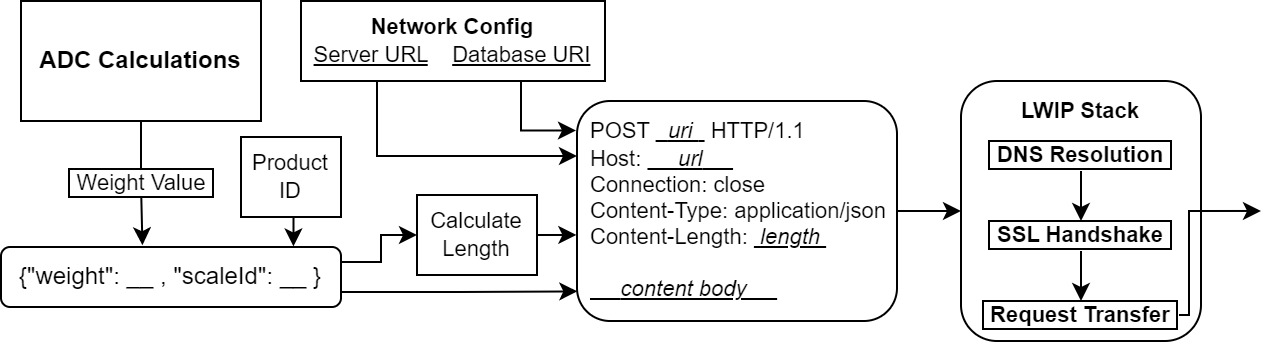
\includegraphics[width=\textwidth]{final-report/assets/network stack diagram.jpg}
\caption{embedded network stack diagram}
\end{figure}


\section{Backend}
MongoDB was used for the database due to its flexibility, scalability and powerful querying capabilities. Its document-oriented model allows for easy storage and management of data. Each entry in the database is stored as a document, which can be grouped and organised into collections. The project consisted of four collections: dogs, users, weights, and chats. The database schema is shown below in Figure 8.1 and reflects the relationship between the different collections.

\begin{figure}[h]
\centering
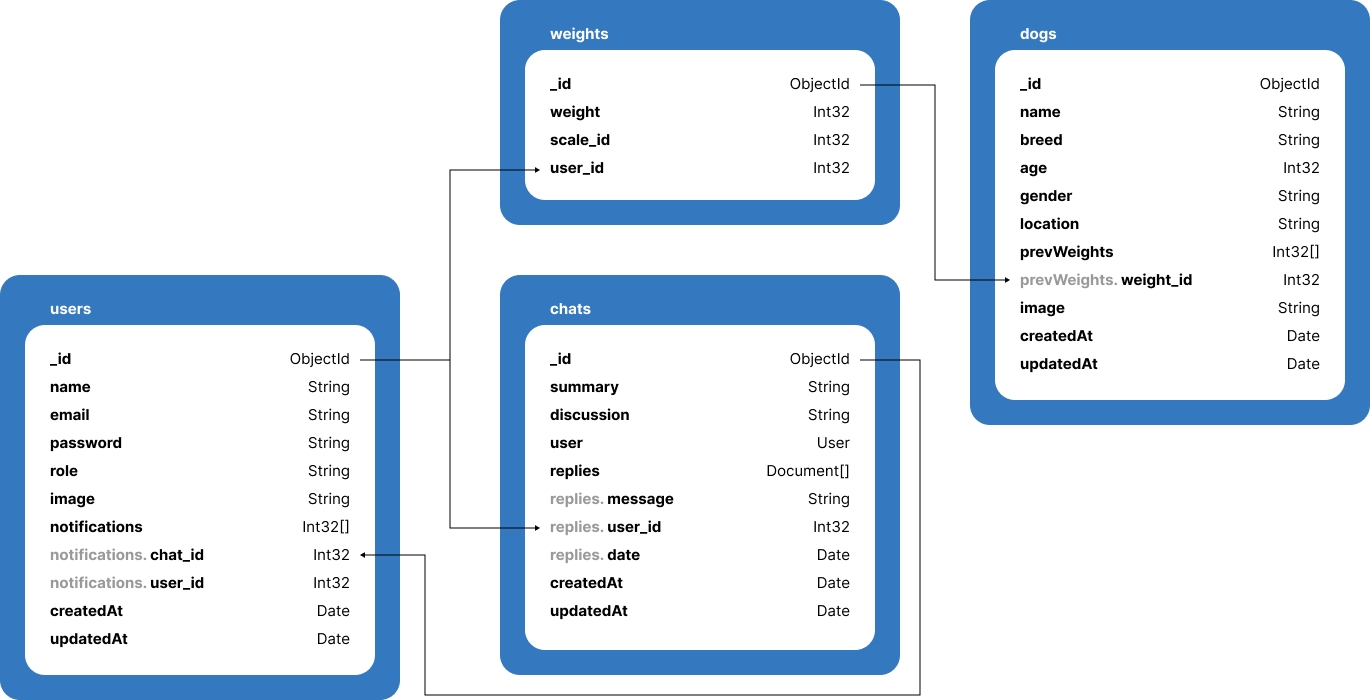
\includegraphics[width=\textwidth]{final-report/assets/databse_schema.png}
\caption{Database Schema}
\end{figure}

We utilised MongoDB’s role based access control where privileges are assigned to roles, ensuring that only authorised users can access the database, restricting unauthorised actions on the database. All users (administrators, vets, and volunteers) have read and write access to animal records and administrators have additional access to staff data. Any attempt to access the database from an external user will be unauthorised.

For user authentication, we used Firebase Authentication using password based accounts. The Firebase SDK was integrated into our application, granting us access to the Firebase Authentication APIs and its built in functionalities. Firebase handled all registrations of new accounts and the authentication processes for existing users, securely verifying the user’s credentials. Once a user is successfully authenticated, a unique authentication token would be generated which can be used to authorise the user’s access to protected resources within the application.

Node.js and Express.js were used for the backend server, handling the processing and management of data and serving it to the client-side. The server was responsible for receiving and interpreting requests from clients, executing the necessary logic, interacting with the database, and generating appropriate responses. Routes were defined to handle specific endpoints, allowing the server to handle various HTTP methods such as GET, POST, PUT, and DELETE. The server would then construct the response and send it back to the client. A list of the endpoints used within this project can be found in Appendix C.


\section{Frontend}
For the frontend, a website was developed using React, a popular JavaScript library for building user interfaces, and Vite, a fast development server and bundler. The website’s frontend consists of several interconnected pages that provide various functionalities to the users. The design of the user interface can be found in Appendix D.

\textbf{Login Page}\\
The login page is the first page encountered by users. Users can enter their credentials to authenticate their access and log into the application. The backend server, powered by Firebase, generates an authentication token upon successful authentication which is stored in the browser's local storage.

\textbf{Navigation Bar}\\
The navigation bar acts as a central hub for accessing different sections and features of the application. It is prominently positioned at the top of each page, providing quick access to different pages and features. It includes links to the dashboard, chat, and sign out options as well as the additional manage users section for administrators. The current user role is stored and this determines the appropriate navigation bar layout.

\textbf{Dashboard Page}\\
The dashboard page is the main page of the website, providing an overview of all the dogs currently in the system. It also includes features such as sort and search to ease user experience. Users can also add new dogs to the system by filling out a form. The backend server fetches all the necessary data from the database, allowing it to be displayed via the web interfavce.

\textbf{Dog Details Page}\\
The dog details page provides comprehensive information for a selected dog. This includes the dog's previous weights which is displayed as both a table and graph, allowing staff to easily visualise and track weight changes over time. All the data is retrieved via the backend server and is used to populate the dog's details and previous weights information.

\textbf{Add Weight Page}\\
The add weight page enables users to input and record weight data for a selected dog. Users must select the scaleID and proceed to the \textit{Add Data: Processing Page}. The selected scaleID is stored and serves as an identifier for the scale used to measure the dog's weight.

\textbf{Add Weight: Processing Page}\\
The processing page offers users a visual indication of the weight recording process. It displays real-time feedback by including a dog footprint animation. When a new weight is added to the database, the page will automatically proceed to the results page.

\textbf{Add Weight: Results Page}\\
The results page provides an overview of the weight measurements recorded during the weighing session. From the displayed data, users can select the weight to be added for the dog. Additionally, if users wish to reweigh the dog, they have the option to re-initiate the weighing process. The previous weight will also be kept, providing the user the option to select the most reasonable weight. All the weight recordings for the current weighing sessions is stored and once the user selects a weight to be added, it is added to the selected dog and the remaining weights are cleared from the database.

\textbf{Chat Page}\\
The chat page is a dedicated forum for communication among users, facilitating discussions and information sharing. Users can initiate discussions, reply to questions and participate in ongoing conversations. Current chat discussions can be organised by searching for certain topics or users. All relevant data including chat summaries, discussions, and replies are stored in the database.

\textbf{Notification Centre}\\
The notification centre stores all the chat notifications for the current user, allowing them to stay updated on interactions in their discussions. A user receives a notification when another user replies to a conversation they have initiated. All notification data is stored in the database.

\textbf{Manage Users Page}\\
The manage users page can only be authorised by administrators. Administrators can view, search, and filter through all the users currently in the system. New users can also be added by filling out a form. All user data is stored in the database and any newly collected data upon the creation of a new user is also added to the database.

\textbf{Sign Out}\\
The sign our popup securely logs users out of the application. by clicking this link, users terminate their current session. Firebase Authentication handles the sign out process by updating the sessions status and invalidating the current user's authentication token.

\subsection{Dataflow}
The frontend communicates with the backend via HTTP requests and responses. The user interacts with the website and its various components where each component has its own associated functionality. For an action, React sends an HTTP request to the backend server with the required parameters. In the backend, Express.js defines routes that map to specific URL endpoints, handling all incoming requests from the frontend and containing the necessary logic to process the request. The backend then communicates with the database to store and retrieve the requested data. Once the backens has successfully processed the request and retrieved or manipulated the relevant data, it generates an appropriate response and sends this back to the frontend. Upon receiving this response, the frontend UI is updated accordingly.

\begin{figure}[h]
\centering
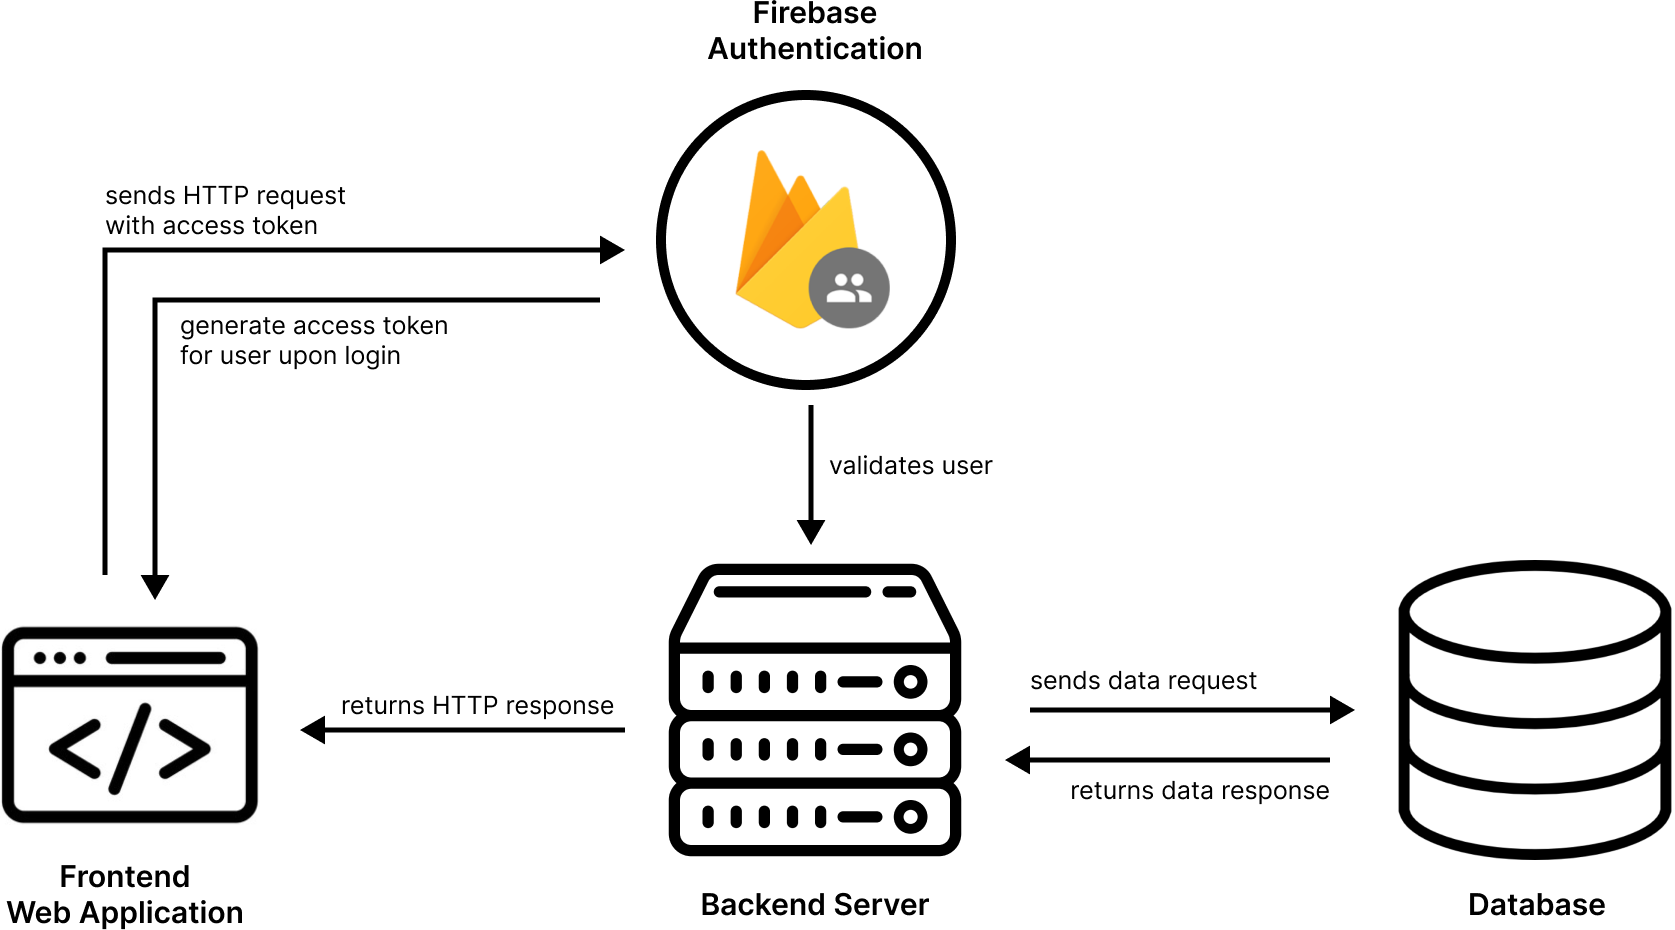
\includegraphics[width=\textwidth]{final-report/assets/dataflow.png}
\caption{Dataflow}
\end{figure}

\textbf{User Sign Up}
\begin{itemize}
    \item Frontend: Admin fills out a registration form to add a new user and submits it.
    \item Backend: Firebase validates the registration request, and securely stores the user’s email and password in its authentication system. It also generates a unique user identifier for the user and sends a response back to the frontend, notifying the user of success or failure of the registration process. Once validated, the user’s information is securely stored in the MongoDB database.
\end{itemize}

\textbf{User Login}
\begin{itemize}
    \item Frontend: User enters the login credentials and submits the login form.
    \item Backend: Firebase verifies the credentials against the stored user data, and generates an authentication. The token is sent back to the frontend as a response.
\end{itemize}

\textbf{User Sign Out}
\begin{itemize}
    \item Frontend: User clicks on the \textit{Sign out} button.
    \item Backend: Firebase receives the sign-our request and invalidates the user’s authentication session. Any active authentication tokens associated with the user are cleared. A response is sent back to the frontend indicating a successful sign out.
\end{itemize}

\textbf{Data Retrieval}
\begin{itemize}
    \item Frontend: User navigates to a page that requires data. Pages include the dashboard page, chat page, manage users page, and dog details page.
    \item Backend: Express.js receives the request, queries the MongoDB database for the requested data, and retrieves the relevant information. The data is sent back to the frontend as a response.
\end{itemize}

\textbf{Data Modification}
\begin{itemize}
    \item Frontend: User performs an action that modifies data. Actions include add dog, add weight, add user, add chat, and add reply.
    \item Backend: Express.js receives the request, validates and processes the incoming data, and updates the MongoDB database accordingly. A response indicating the success or failure of the operation is sent back to the frontend.
\end{itemize}

\textbf{Error Handling}
\begin{itemize}
    \item Frontend: An error occurs during a request.
    \item Backend: Express.js detects the error, generates an appropriate error response, and sends it back to the frontend for display or handling.
\end{itemize}

\section{Requirements Compliance}
To demonstrate compliance with the concurrent connections and data storage requirements, our implementation was thoroughly tested and evaluated through a combination of manual checking and verification procedures. Although automated frontend and backend testing was not conducted, manual testing provided valuable insights into the system’s performance, concurrency handling and data storage integrity.

\subsection{Concurrent Connections Testing}
To ensure the system’s ability to handle concurrent connections, we conducted manual testing using the following approach:
\begin{itemize}
    \item Multiple users were simulated to access the application simultaneously.
    \item Through careful observation and analysis, we validated that the system remained stable and responsive under various concurrent connection scenarios.
\end{itemize}

\subsection{Data Storage Testing}
To evaluate compliance with data storage requirements and ensure data integrity, the following manual testing approach was adopted:
\begin{itemize}
    \item Rigorous manual checks were performed to validate that data was stored correctly and consistently across the frontend and backend components.
    \item We cross-checked data across different application pages to ensure consistency and accuracy of stored data.
\end{itemize}
